\documentclass[12pt,a4paper]{article}
\usepackage[UTF8]{ctex}     %先引入ctex
\usepackage[utf8]{inputenc} %再引入inputenc
\usepackage{graphicx}
\usepackage{geometry}
\usepackage{xcolor}
% \usepackage{lazylatex}
\usepackage{amsmath}
\usepackage{enumerate}
\usepackage{caption}
\usepackage{listings}
\captionsetup[lstlisting]{labelfont=bf,justification=justified}

\usepackage{tikz}
\usepackage{pgfplots}
\pgfplotsset{compat=1.17}
\usepackage{appendix}

\graphicspath{{img/}}
% 边距
\geometry{left=2.0cm,right=2.0cm,top=2.0cm,bottom=3.0cm}
% 大题
\newenvironment{problems}{\begin{list}{}{\renewcommand{\makelabel}[1]{\textbf{##1}\hfil}}}{\end{list}}
% 小题
\newenvironment{steps}{\begin{list}{}{\renewcommand{\makelabel}[1]{##1.\hfil}}}{\end{list}}
% 答
\providecommand{\ans}{\textbf{答}:~}
% 解
\providecommand{\sol}{\textbf{解}.~}

\usepackage[colorlinks,linkcolor=blue]{hyperref}
\usepackage{bookmark}
\providecommand{\code}[2]{\lstinputlisting[language=#2,caption=\href{run:#1}{\ttfamily #1}]{#1}}
\providecommand{\img}[1]{\includegraphics[width=0.88\textwidth]{#1}}

% listings
\definecolor{grey}{rgb}{0.8,0.8,0.8}
\definecolor{darkgreen}{rgb}{0,0.3,0}
\definecolor{darkblue}{rgb}{0,0,0.3}
\lstset{%
    % numbers=left, %行号
    % numberstyle=\tiny\color{grey},
    showstringspaces=false,
    showspaces=false,%
    tabsize=4,%
    frame=shadowbox,%
    basicstyle={\ttfamily\scriptsize},%
    keywordstyle=\color{blue!80!black}\bfseries,%
    identifierstyle=,%
    commentstyle=\color{green!50!blue}\itshape,%
    stringstyle=\color{green!50!black},%
    rulesepcolor=\color{gray!20!white},
    breaklines,
    columns=flexible,
    extendedchars=false,
    %mathescape=true,
}

\begin{document}
\title{\normalsize \underline{操作系统(D)}\\\LARGE 项目 6}
\author{李子龙 518070910095}
\date{\today}
\maketitle

\textbf{银行家算法}
\begin{problems}
    \item[一] \textbf{输入框架}
    
    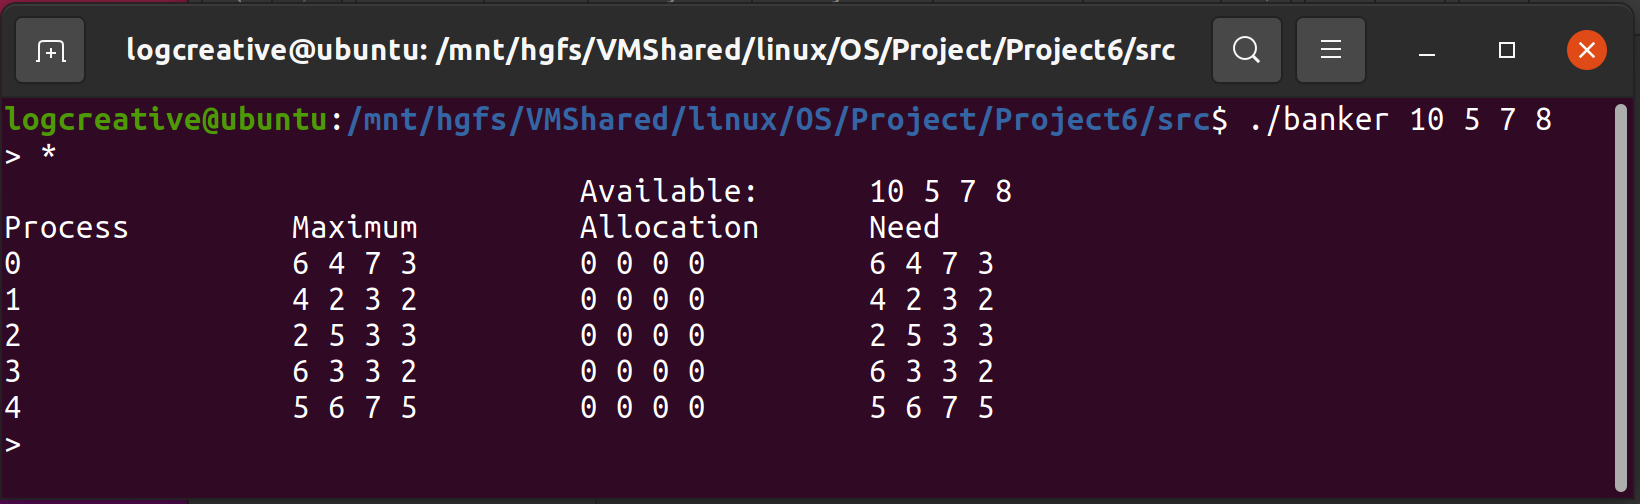
\includegraphics[width=0.88\textwidth]{input.png}

    首先需要读取可用资源和最大使用资源数。使用了 UNIX 系统中 \verb"strsep()" 函数按照 \verb"," 分割输入行。初始时:
    \begin{align*}
        \text{\sffamily maximum}_i &= \text{\sffamily need}_i \\
        \text{\sffamily allocation}_i &=0
    \end{align*}
    \begin{lstlisting}[language=c]
    for(int i = 0; i< NUMBEROFRESOURCES; ++i)
    available[i] = atoi(argv[i+1]);
    
    FILE *in;
    char *temp;
    char customer[MAXLINE];

    in = fopen("info.txt","r");

    for(int i = 0; i<NUMBEROFCUSTOMERS; ++i){
        if(fgets(customer,MAXLINE,in)==NULL){
            fprintf(stderr,"Read file error!\n");
            return -1;
        }
        temp = strdup(customer);

        for(int j = 0; j<NUMBEROFRESOURCES; ++j){
            int maxres = atoi(strsep(&temp,","));
            need[i][j] = maxres;
            maximum[i][j] = maxres;
            allocation[i][j] = 0;
        }
        
        free(temp);
    }

    fclose(in);
    \end{lstlisting}

    之后,仿照命令行的输入设定输入循环。如果输入 \verb"*",则显示系统当前的状态。

    \begin{lstlisting}[language=c]
    char command[2];
    fprintf(stdout,"> ");
    while(fscanf(stdin,"%s",command)!=EOF){
        if (strcmp(command,"RQ")==0){
            int customer_num;
            fscanf(stdin, "%d", &customer_num);
            int request[NUMBEROFRESOURCES];
            for(int j = 0; j < NUMBEROFRESOURCES; ++j)
                fscanf(stdin, "%d", &request[j]);
            if(request_resources(customer_num, request))
                fprintf(stdout, "RQ Denied.\n");
            else fprintf(stdout, "RQ Success.\n");
        } else if (strcmp(command,"RL")==0){
            int customer_num;
            fscanf(stdin, "%d", &customer_num);
            int release[NUMBEROFRESOURCES];
            for(int j = 0; j < NUMBEROFRESOURCES; ++j)
                fscanf(stdin, "%d", &release[j]);
            release_resources(customer_num, release);
            fprintf(stdout, "RL Complete.\n");
        } else if (strcmp(command,"*")==0){
            fprintf(stdout, "\t\t\t\tAvailable: \t");
            for(int j = 0; j<NUMBEROFRESOURCES; ++j)
                fprintf(stdout, "%d ", available[j]);
            fprintf(stdout, "\n");
            fprintf(stdout,"Process\t\tMaximum\t\tAllocation\tNeed\n");
            for(int i = 0; i < NUMBEROFCUSTOMERS; ++i){
                fprintf(stdout, "%d\t\t", i); 
                for(int j = 0; j < NUMBEROFRESOURCES; ++j)
                    fprintf(stdout, "%d ", maximum[i][j]);
                fprintf(stdout, "\t");
                for(int j = 0; j < NUMBEROFRESOURCES; ++j)
                    fprintf(stdout, "%d ", allocation[i][j]);
                fprintf(stdout, "\t");
                for(int j = 0; j < NUMBEROFRESOURCES; ++j)
                    fprintf(stdout, "%d ", need[i][j]);
                fprintf(stdout, "\n");
            }
        }
        fprintf(stdout,"> ");
    }

    return 0;
    \end{lstlisting}
    \item[二] \textbf{请求数据}
    
    如果存在死锁,请求将会被拒绝。

    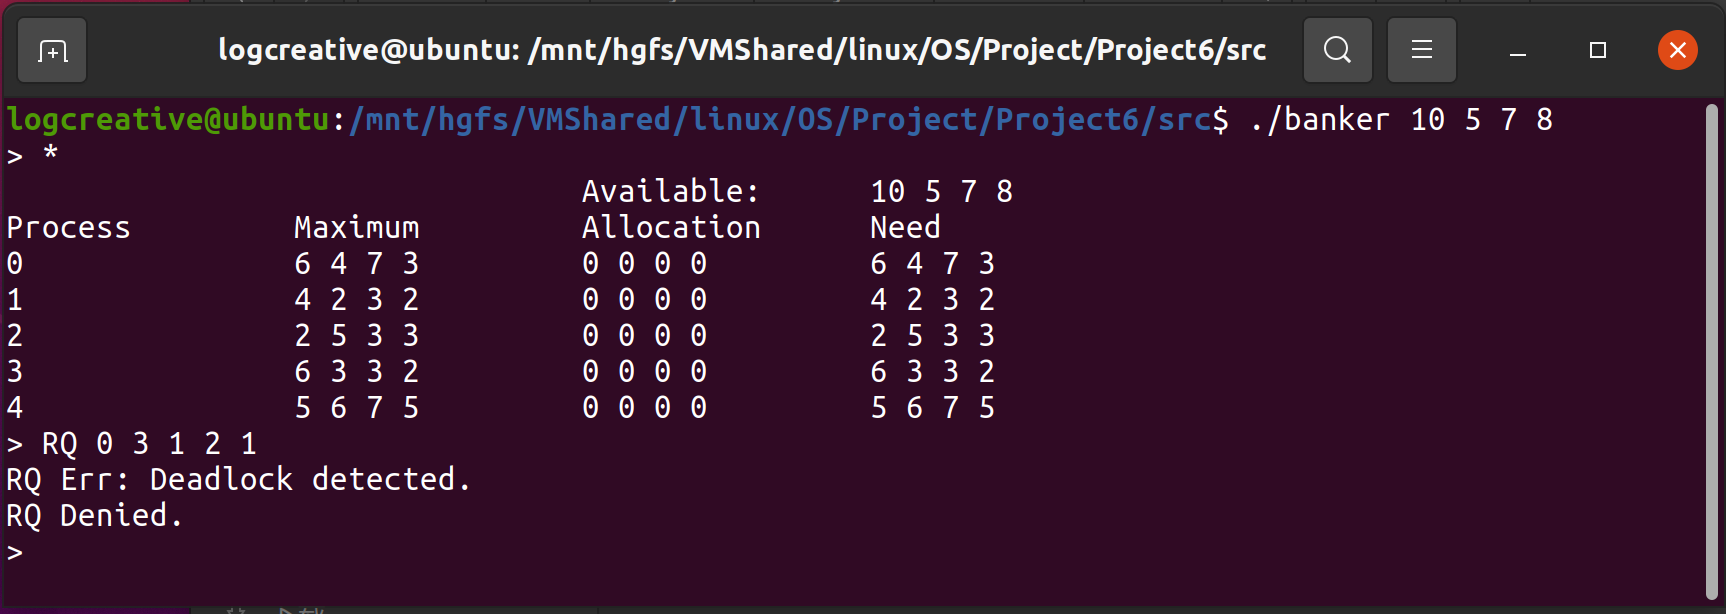
\includegraphics[width=0.7\textwidth]{RQd.png}

    如果请求了过多的资源,超出了自身的最大值,就会有超限的错误。

    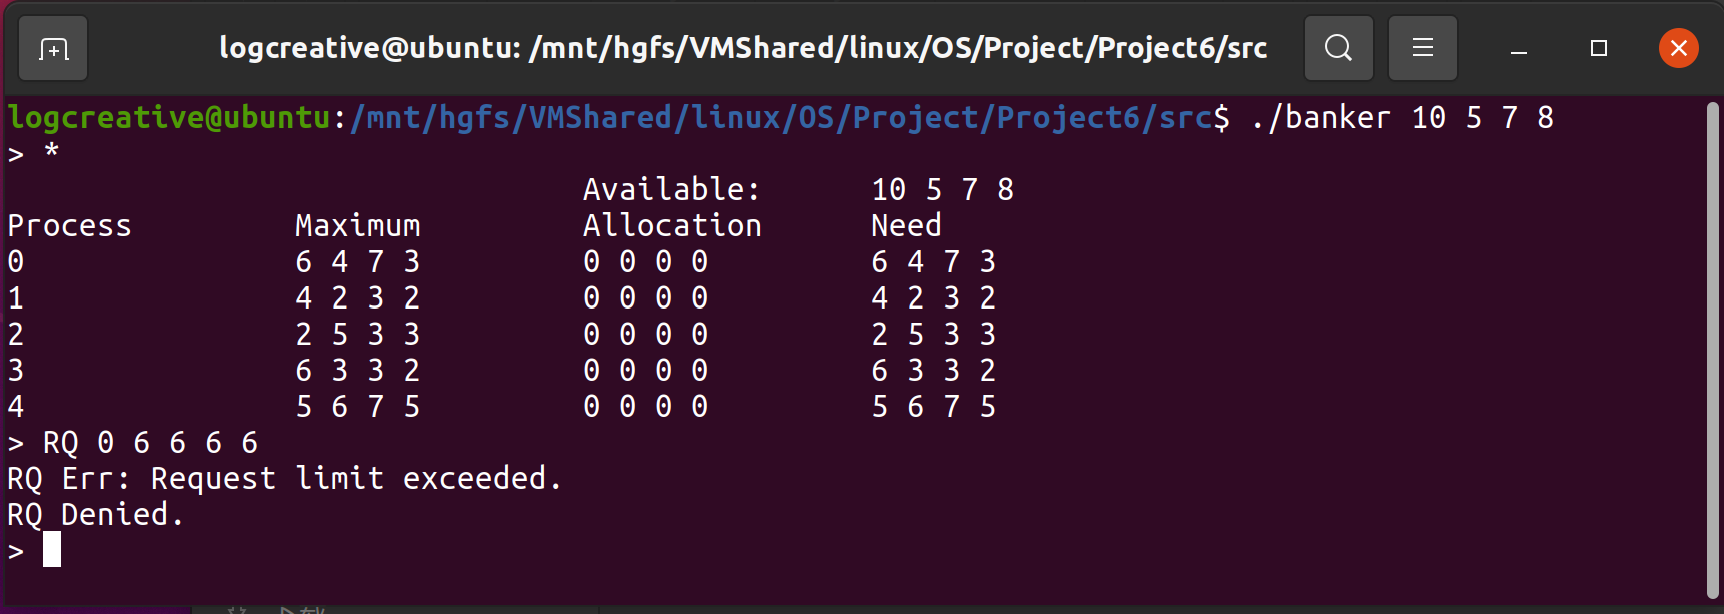
\includegraphics[width=0.7\textwidth]{RQe.png}

    如果请求的资源多于目前可用资源,就会有资源不足的错误。

    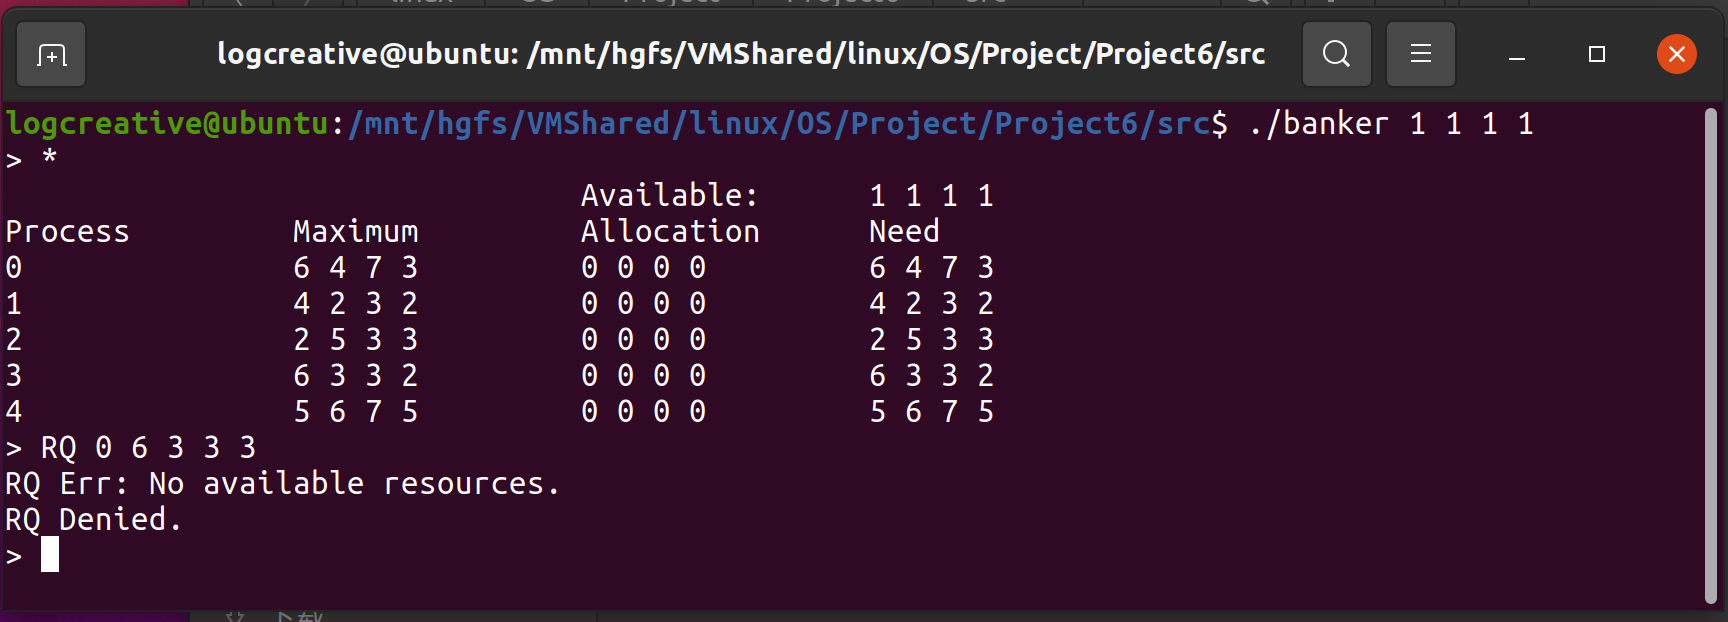
\includegraphics[width=0.7\textwidth]{RQa.png}
    
    如果不存在死锁,请求将会被执行,相关数据将会被刷新。

    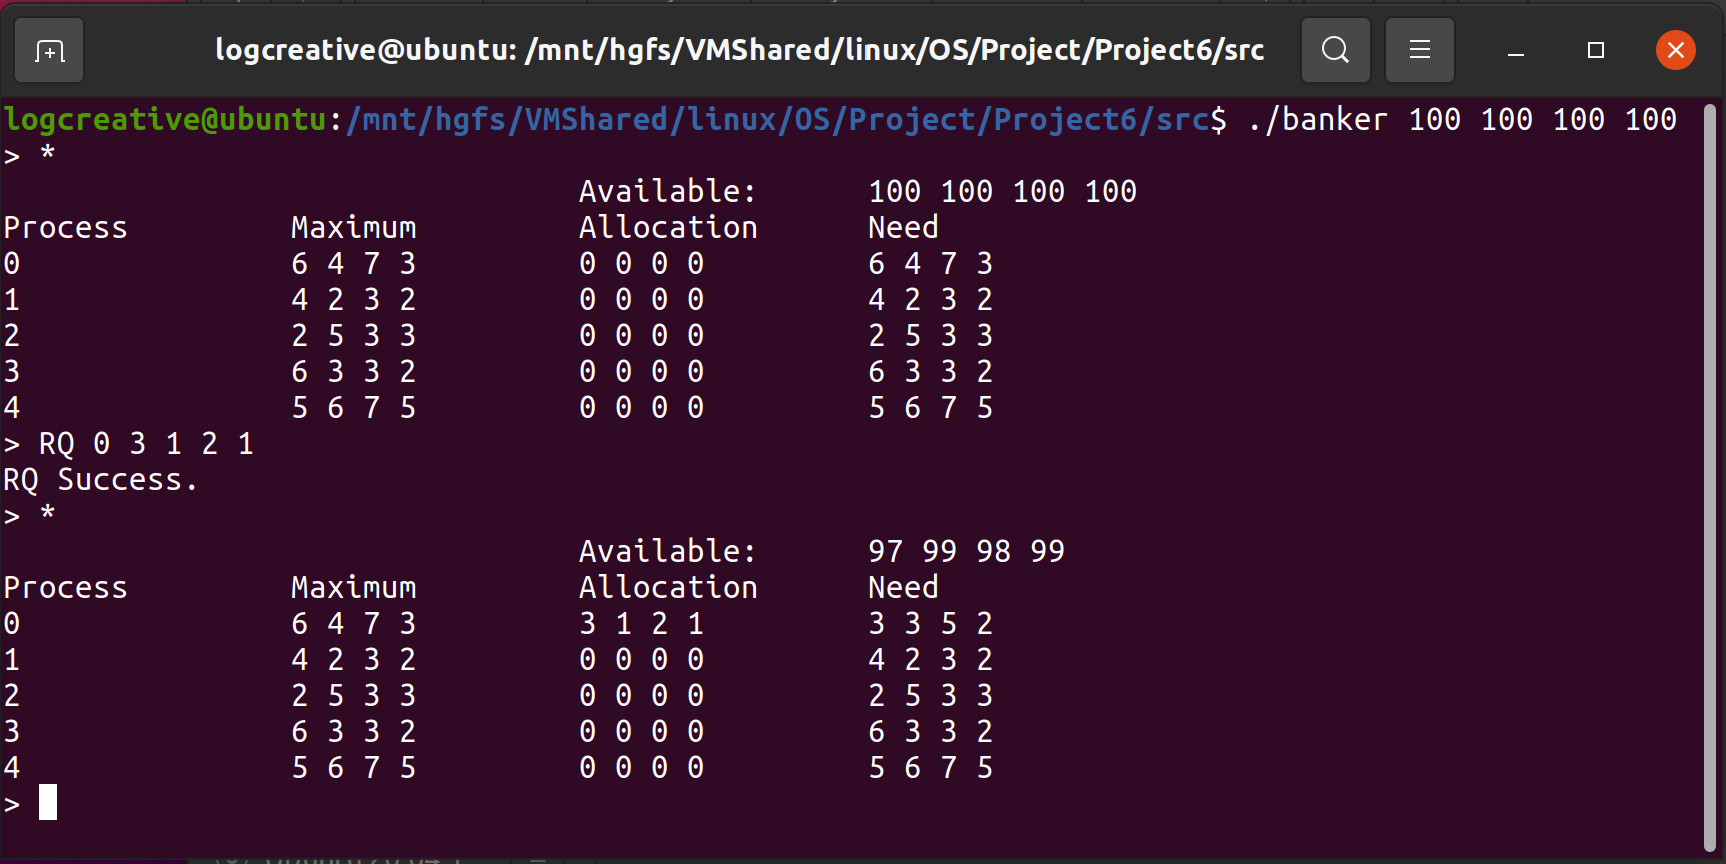
\includegraphics[width=0.7\textwidth]{RQs.png}

    请求函数使用了银行家算法。初始时进行平凡情况的判定,以自起始时弹出错误:
    \begin{lstlisting}[language=c]
    int request_resources(int customer_num, int request[]){
        for(int j = 0; j < NUMBEROFRESOURCES; ++j){
            if(allocation[customer_num][j] + request[j] > maximum[customer_num][j]){
                fprintf(stderr, "RQ Err: Request limit exceeded.\n");
                return 1;
            }
            if(request[j]>available[j]){
                fprintf(stderr, "RQ Err: No available resources.\n");
                return 1;
            }
        }
    \end{lstlisting}

    然后进行假设分配,将可用情况在一个新的数组 \verb"allocation_pre" 中存储。之后会使用 \verb"finish" 数组存储任务的完成情况。
    \begin{lstlisting}[language=c]
        // Fake allocation
        int available_pre[NUMBEROFRESOURCES];
        for(int j = 0; j < NUMBEROFRESOURCES; ++j){
            allocation[customer_num][j] += request[j];
            need[customer_num][j] -= request[j];
            available_pre[j] = available[j] - request[j];
        }
        
        int finish[NUMBEROFCUSTOMERS];
        for(int i = 0; i < NUMBEROFCUSTOMERS; ++i){
            int finish_flag = 1;
            for(int j = 0; j < NUMBEROFRESOURCES; ++j)
                if(need[i][j] > 0)
                    finish_flag = 0;
            finish[i] = finish_flag;
        }
    \end{lstlisting}

    之后就是标准的银行家算法,如果找到了候选者就会继续循环,否则退出循环。候选者的条件两条需要同时满足:(1)未完成;(2)需要的资源可以被当下的可用资源满足。满足后就会更新可用资源的数据。
    \begin{lstlisting}[language=c]
        int found = 0;
        do {
            found = 0;
            for(int i = 0; i < NUMBEROFCUSTOMERS; ++i){
                if(!finish[i]){
                    int next = 1;
                    for(int j = 0; j < NUMBEROFRESOURCES; ++j)
                        if(need[i][j] > available_pre[j]){
                            next = 0;
                            break;
                        }
                    if(!next) continue;
                    finish[i] = 1;
                    for(int j = 0; j < NUMBEROFRESOURCES; ++j)
                        available_pre[j] += allocation[i][j];
                    found = 1;
                    break;
                }
            }
        } while (found);
    \end{lstlisting}

    如果退出循环后依然有未完成的任务,则存在死锁,对分配进行回滚操作。如果可行就只需要修改 \textsf{available} 数组的相关值。
    \begin{lstlisting}[language=c]
        int all_finish_flag = 1;
        for(int i = 0; i < NUMBEROFCUSTOMERS; ++i)
            if(!finish[i])
                all_finish_flag = 0;
        if(!all_finish_flag){
            // fallback
            for(int j = 0; j < NUMBEROFRESOURCES; ++j){
                allocation[customer_num][j] -= request[j];
                need[customer_num][j] += request[j];
            }
            fprintf(stderr, "RQ Err: Deadlock detected.\n");
            return 1;
        }
    
        for(int j = 0; j < NUMBEROFRESOURCES; ++j)
            available[j] -= request[j];
        return 0;
    }
    \end{lstlisting}

    \item[三] 资源释放
    
    资源正常释放,\textsf{Maximum} 和 \textsf{Allocation} 的值都会修改。

    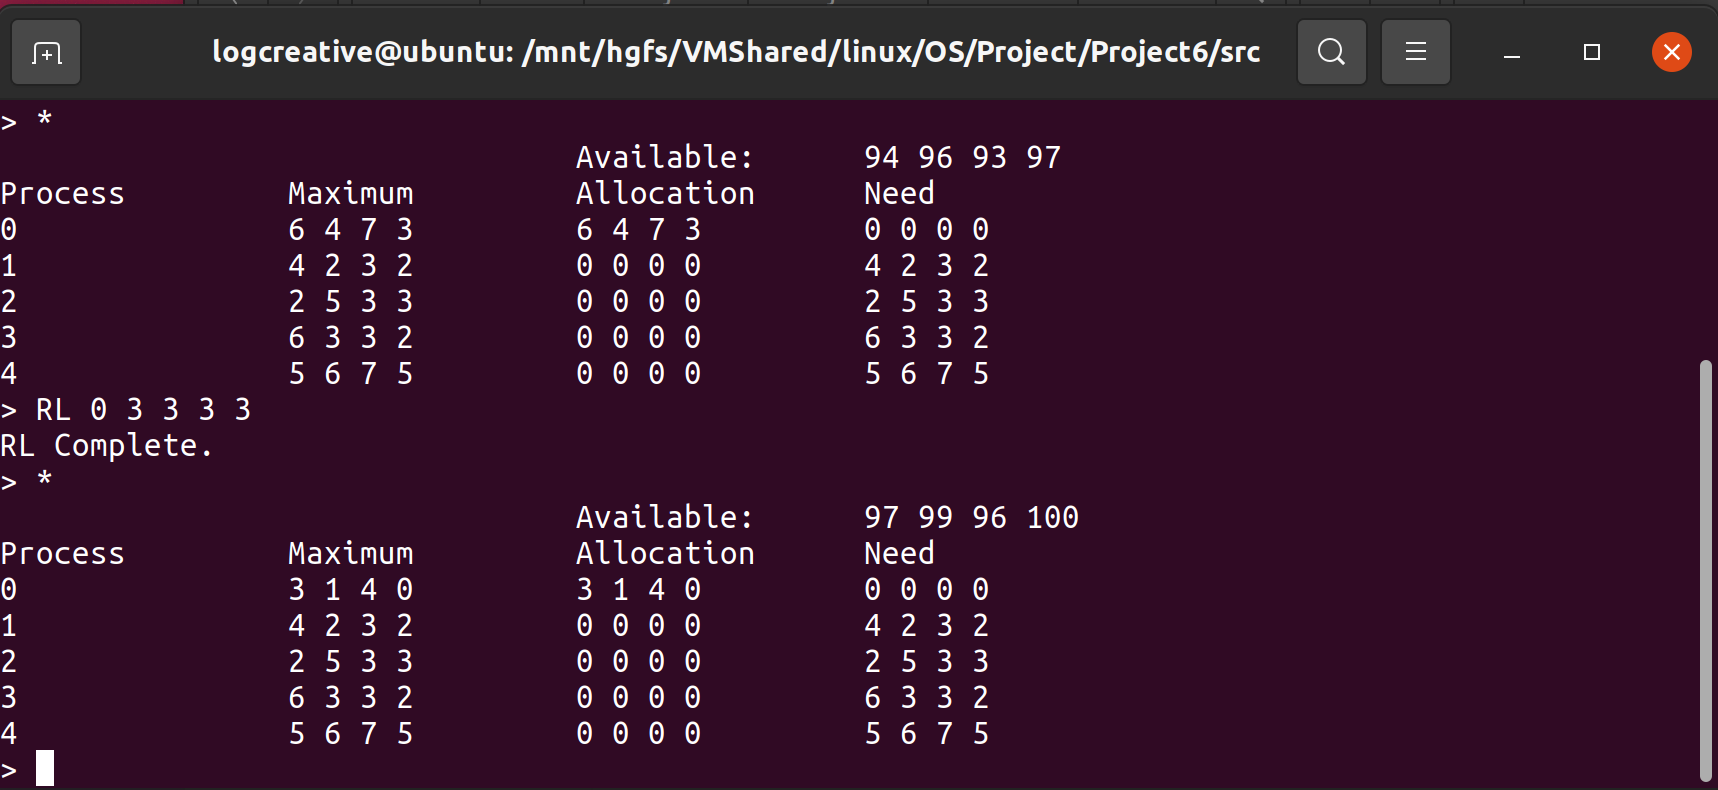
\includegraphics[width=0.7\textwidth]{RLs.png}

    如果释放不了这么多的资源,就会释放该资源能释放的最大值,并弹出警告。

    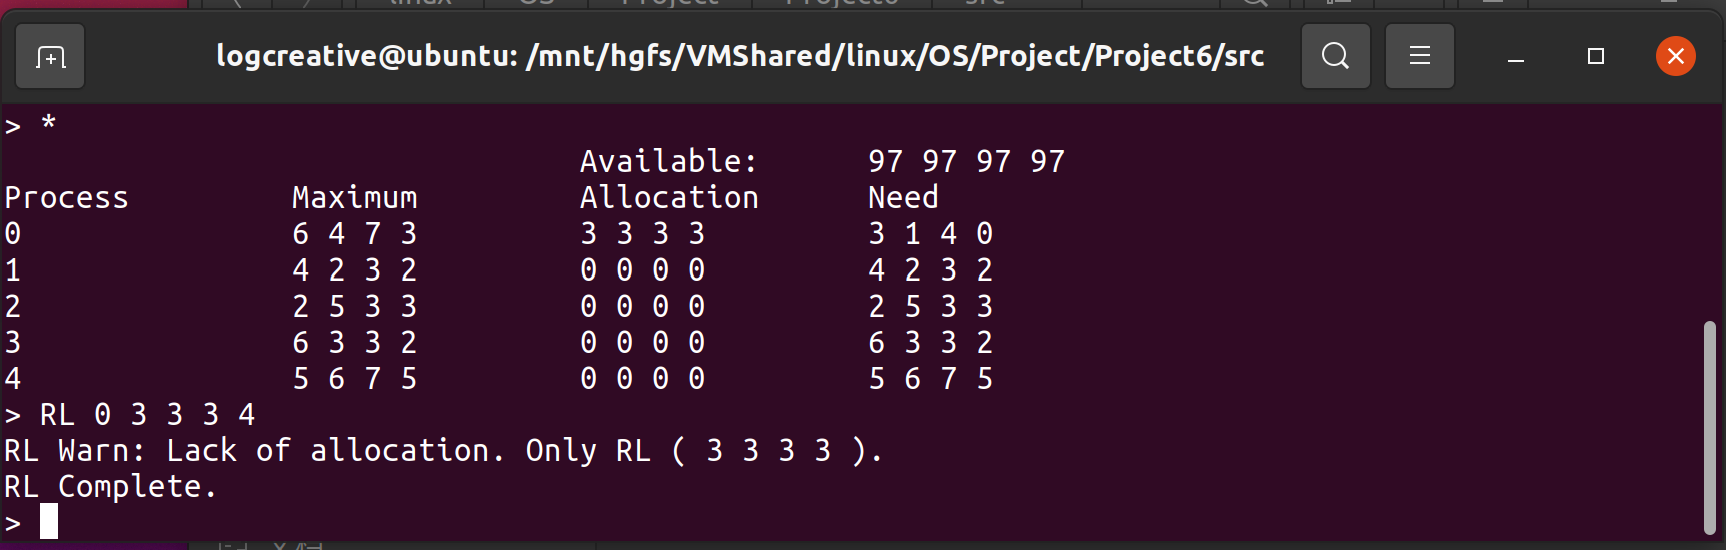
\includegraphics[width=0.7\textwidth]{RLo.png}

    如果资源全部释放完毕,会提示该进程已经结束。

    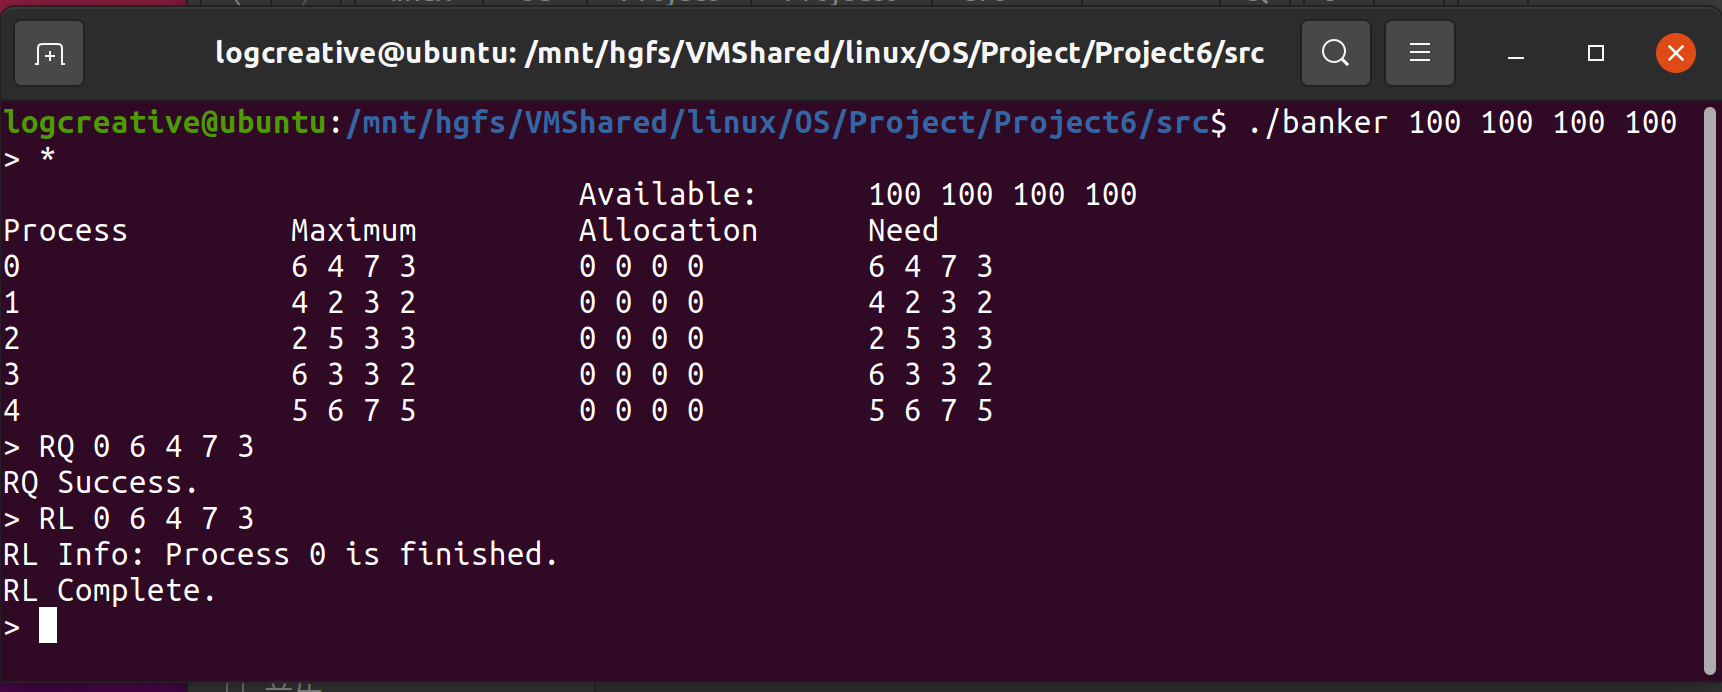
\includegraphics[width=0.7\textwidth]{RLf.png}
    
    释放函数的定义如下:只要释放就认为这些资源已经不需要了,将会从最大值中减去,该任务不能再请求更多的资源。
    \begin{lstlisting}[language=c]
    void release_resources(int customer_num, int release[]){
        int real_release[NUMBEROFRESOURCES];
        int warn_flag = 0;
        for(int j = 0; j < NUMBEROFRESOURCES; ++j){
            if(release[j] > allocation[customer_num][j]){
                real_release[j] = allocation[customer_num][j];
                warn_flag = 1;
            }
            else real_release[j] = release[j];
            allocation[customer_num][j] -= real_release[j];
            maximum[customer_num][j] -= real_release[j];
            available[j] += real_release[j];
        }
        if(warn_flag){
            fprintf(stderr, "RL Warn: Lack of allocation. Only RL ( ");
            for(int j = 0; j < NUMBEROFRESOURCES; ++j)
                fprintf(stdout, "%d ", real_release[j]);
            fprintf(stdout, ").\n");
        }
        int fin_flag = 1;
        for(int j = 0; j < NUMBEROFRESOURCES; ++j)
            if(maximum[customer_num][j]>0)
                fin_flag = 0;
        if(fin_flag)
            fprintf(stdout, "RL Info: Process %d is finished.\n", customer_num);
        }
    }
    \end{lstlisting}
\end{problems}

\begin{appendices}
    \section{全部代码}
    \code{src/Makefile}{}
    \code{src/banker.c}{c}
    \code{src/info.txt}{}
\end{appendices}

\end{document}
